% !TEX root = ../thesis.tex

\chapter{AVPipe的测试与评估}

在这一章中,我们将展示由AVPipe构建的不同视频流处理任务。并通过对具体视频处理任务在不同平台的运行来展示AVPipe提供的性能优化。

\section{测试任务}
本小节会对我们所使用的视频处理任务进行简单介绍。以下模型/处理流程都是对一些出名的开源项目在AVPipe框架下的实现。
% \subsection{视频物体识别任务} % TODO

\subsection{视频人体姿态估计任务}
人体姿态估计是指识别图像中人体各个关节点的位置。我们基于Sun et al.提出的HRNet(High Resolution Network)\cite{sun2019deep}来构建本任务。HRNet是一个多层级的深度CNN模型,它主要利用了多尺度图像中的空间结构信息来提高检测精度。我们在图\ref{fig:pose_dag}已经展示了基于HRNet的人体检测估计的数据处理流程。在这一处理流程中,预处理后的图像数据会被送入HRNet进行推理,其输出是一个包含人体关键点信息的热图(heat map)张量,在后处理过程中,我们会对这个原始输出行进高斯滤波(filter),多通道峰值选择(maxPred)等操作,最终获得一个与输入图片相对应的关键点坐标列表。在进行最后的输出渲染时,我们只显示预测置信度高于于预设阈值的关键点。本任务中各个步骤之间的依赖关系较为简单,
可以将该处理过程分为预处理,神经网络推理,后处理三部分进行多线程流水线优化。这也正是AVPipe自动多线程优化所得的结果(图\ref{fig:pose_dag})。在神经网络的推理上,我们使用OpenVINO作为HRNet的推理引擎,并且将高斯滤波(filter)看作是单层卷积网络由TorchScript进行实现。方便起见,我们会在后续测试中将该视频处理任务简称为Pose。

\subsection{视频手部检测与追踪任务}
与人体姿态估计任务类似,手部检测与追逐是指检测出图像的人手,并对手部的动作进行捕捉。在这里我们采用了Google提出的手部追踪处理流程\cite{mediapipe_hand}。图\ref{fig:hand_dag}展示了该处理流程在AVPipe中的可视化。
该处理流程用到了两个CNN模型分别用来做手部检测(PalmCNN)与手部关键点定位(HandCNN)。首先经过预处理的图像数据会送入PalmCNN,PalmCNN是一个基于SSD(Single Shot MultiBox Detector)\cite{liu2016ssd}模型进行简化的检测模型,在拿到PalmCNN的原始检测结果后,需要通过尺寸缩放(decodeBoxes),非极大值抑制(NMS)等后处理操作获得可以对应原图的手部检测框。在接下来的处理流程中,手部检测结果会根据其对应的检测框进行旋转,剪裁与缩放,构成一批手部位于图像中心的图片,这批图片会在预处理后送入HandCNN进行关键点定位。最后,关键点信息会通过转换(rotateBack)对应回原图中的坐标。\par
为了减少处理过程中的冗余计算,加快流程的处理速度,该手部追踪处理流程还在其检测算法流程上进行了针对视频任务的优化。由于人手在连续视频帧中的位移量一般较小,故可以直接使用上一帧关键点检测结果估计人手在下一帧中出现的位置,从而PalmCNN不必每帧都运行,它只需要在一些关键帧或检测目标丢失时运行。为实现这部处理逻辑,我们在AVPipe中设立了两个自定义的计算模块multiplexer和streamMerger用来选择运行正确的数据源。未将本帧计算结果转播到下一帧去,我们在处理流程中加入了timeUpdate模块,其产生的数据包会被标记为下一帧的时间戳(图\ref{fig:hand_dag}中的虚线箭头),这点也会在建立计算图时由Stream进行必要的特殊初始化。\ref{fig:hand_dag}也展示了该处理任务在4个线程下的划分,该划分将两个CNN放入了两个不同的线程中,线程间不存在局部依赖,
每个线程的耗时都不超过最耗时模块的用时,满足我们对该计算图的优化期望。我们使用ONNX Runtime为该处理流程中的两个神经网络提供优化推理。
在测试过程中,我们会分别对使用了上述算法优化(由Hand-opt表示)和未使用上述算法优化的处理流程(由Hand-raw表示)进行性能测试。

\begin{figure}[!bt]
    \centering
    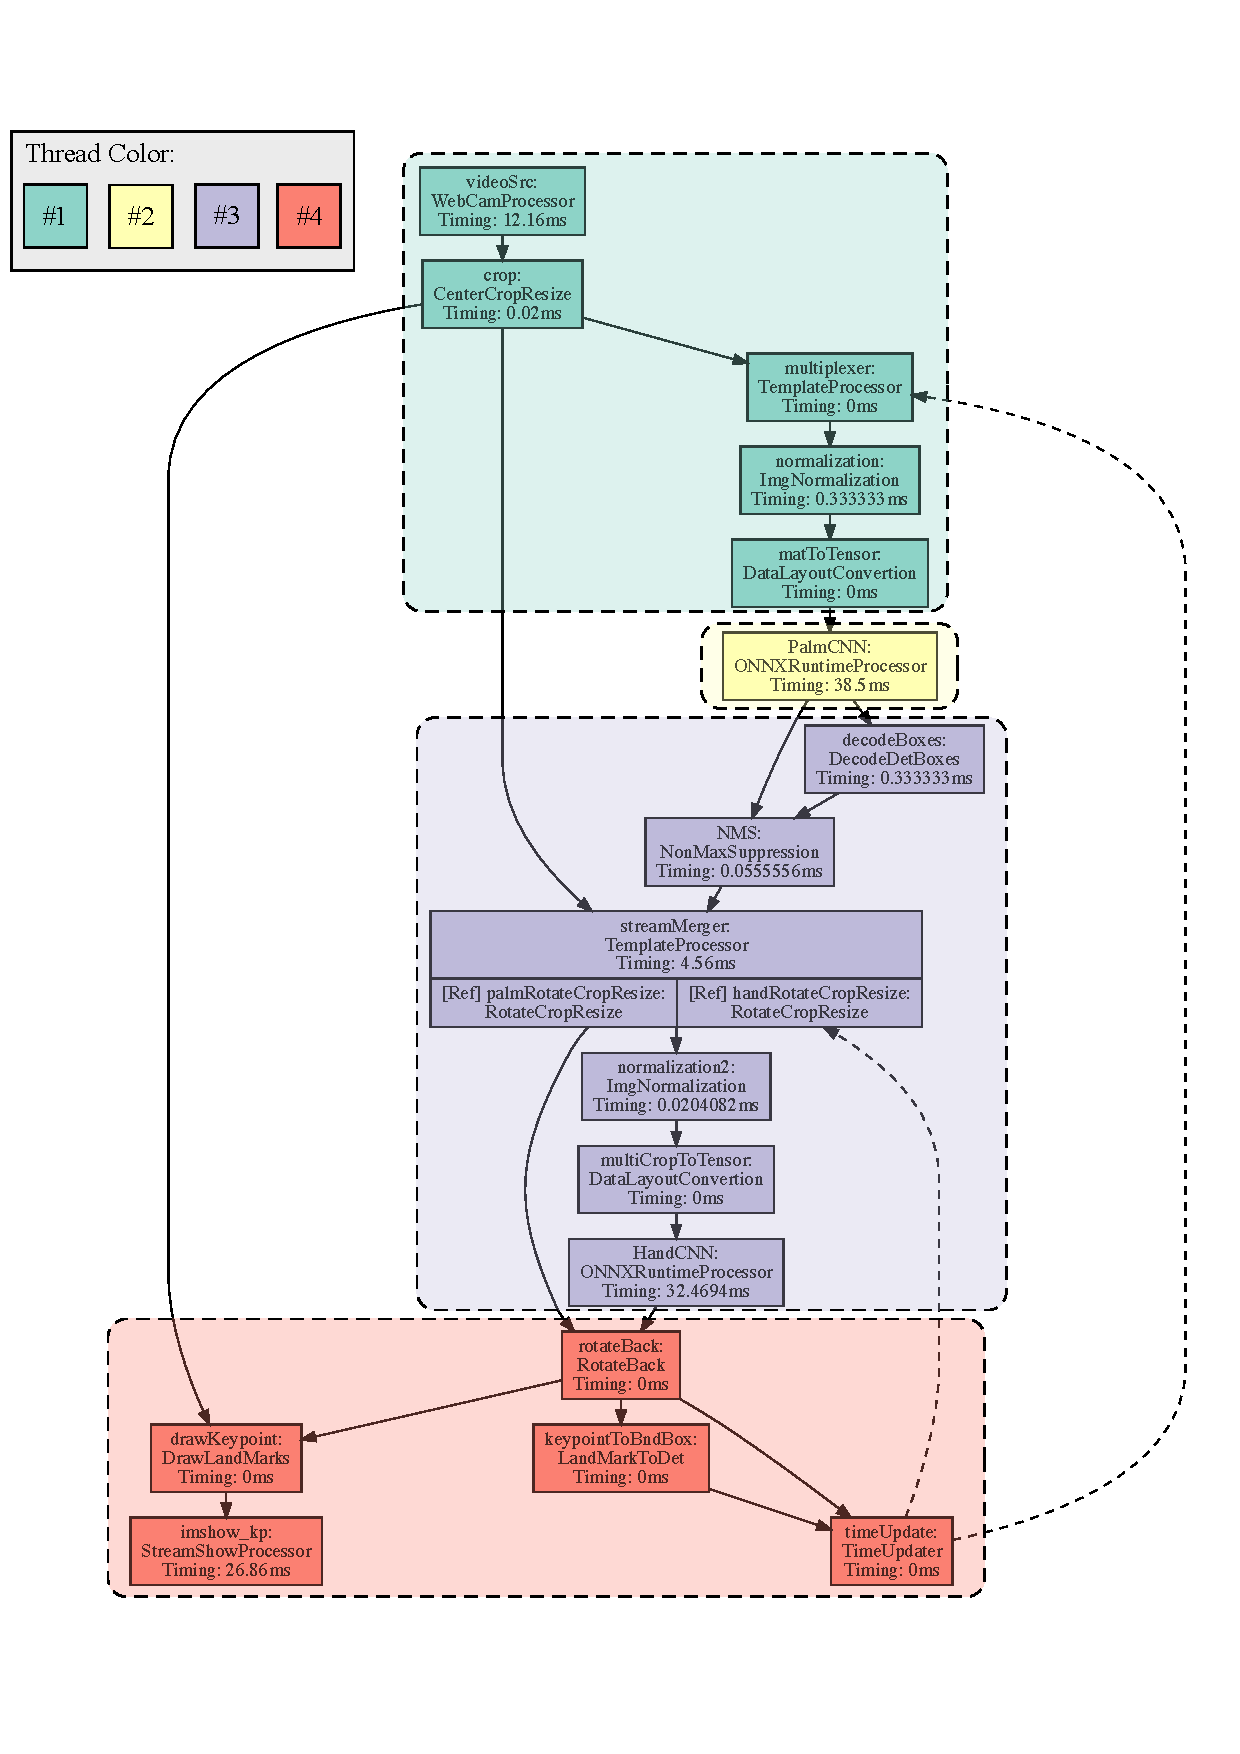
\includegraphics[width=0.7\textwidth]{figure/AVP_multi_hand_tracking.pdf}
    \bicaption[手部追踪任务在AVPipe框架下处理流程的可视化]{手部追踪任务在AVPipe框架下处理流程的可视化。图中虚线连接表示该模块的在本时间戳的输出会在下一时间戳中使用。 由于本图的连接较为复杂,为便于观察,我们没有提供如图\ref{fig:pose_dag}中的Stream可视化,只保留模块间连接。
    节点运行时间信息来自Intel i5-8210Y处理器的MacBook Air的预运行。}{AVPipe visualization of multiple hand tracking video processing task.}
    \label{fig:hand_dag}
\end{figure}

\section{运行环境与参数设置}
目前AVPipe框架完成了对macOS,Linux以及Windows这三大桌面操作系统的支持\footnote{我们会在以后尽可能地提供对移动平台的支持,但这部分并不属于本研究课题所关注的重点。}。同时,由于AVPipe框架的目标设备主要是用户个人的终端,而非高性能的服务器,因此我们选择的macOS和Windows这两个主流平台下的便携笔记本电脑作为测试设备(我们手上持有的计算设备也只能支持我们选择这样的测试设备)。对macOS平台,我们使用了一台MacBook Air,其搭载了,
Intel i5-8210Y双核心处理器;对Windows平台,我们使用了一台ThinkPad X1 Carbon,其搭载了Intel i5 10210U四核心处理器。更多核心数量能为多线程运行带来更好的性能,这一点我们也可通过对比这两款设备的处理速度来进行观察。
为体现AVPipe在多硬件场景下的支持,我们还在后续测试中使用了Intel Neural Compute Stick 2(NCS2)\footnote{\url{https://software.intel.com/content/www/us/en/develop/hardware/neural-compute-stick.html}}这一神经网络加速器,以及Intel的核心显卡进行处理流程的构建。\par

在测试过程中,为了尽可能减少其他因素对运行结果的影响,同一处理任务在不同平台下均使用同一视频文件的前200帧作为输入进行分析。在运行视频处理任务时,我们会尽可能关闭系统中其他正在运行的高资源占用进程。我们在这些视频处理任务中所使用的CNN在未特殊说明的情况下均为全精度(float32)模型,且在进行多线程优化时最大线程数量默认为4.

\section{性能对比分析}

图\ref{fig:stats}展示了我们的测试视频处理任务在不同设备上的运行速度。总的来说,我们的测试视频处理任务可以在这些非高性能便携计算设备上达到高于10帧每秒(FPS)的处理速度,这基本可以实现低帧率视频的实时处理。AVPipe提供的多线程优化,在对比的各组测试中均可以有效地降低视频处理的耗时,下面我们将对此做具体分析。\par

\begin{figure}[htp]
    \centering
    \begin{subfigure}{0.49\textwidth}
    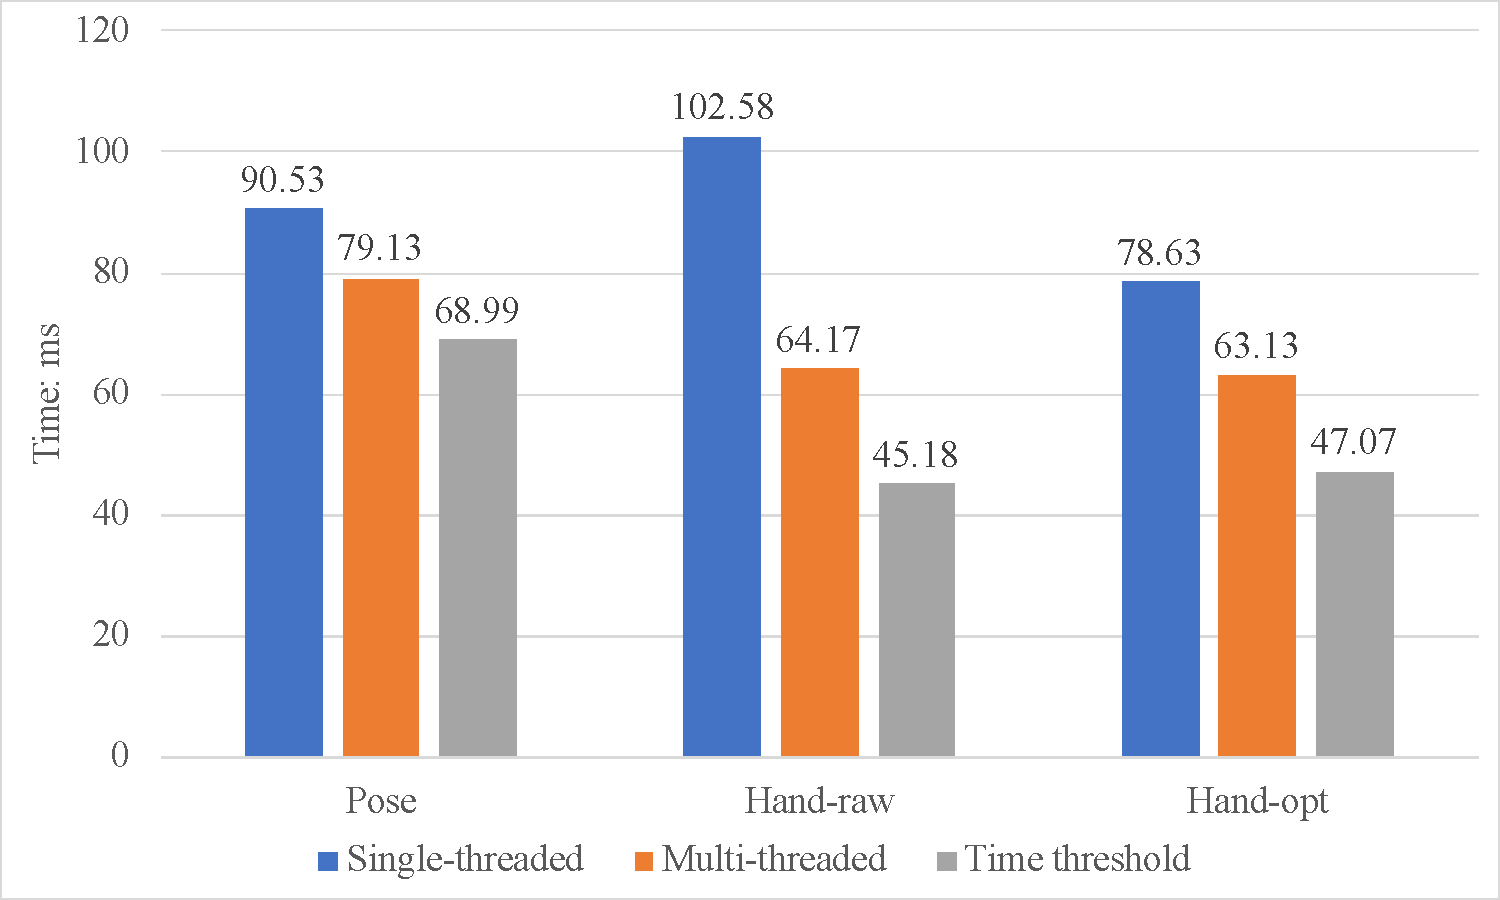
\includegraphics[width=\textwidth]{figure/mac_stats.pdf}
    \caption{MacBook Air, i5 2-Core}
    \end{subfigure}
    \begin{subfigure}{0.49\textwidth}
    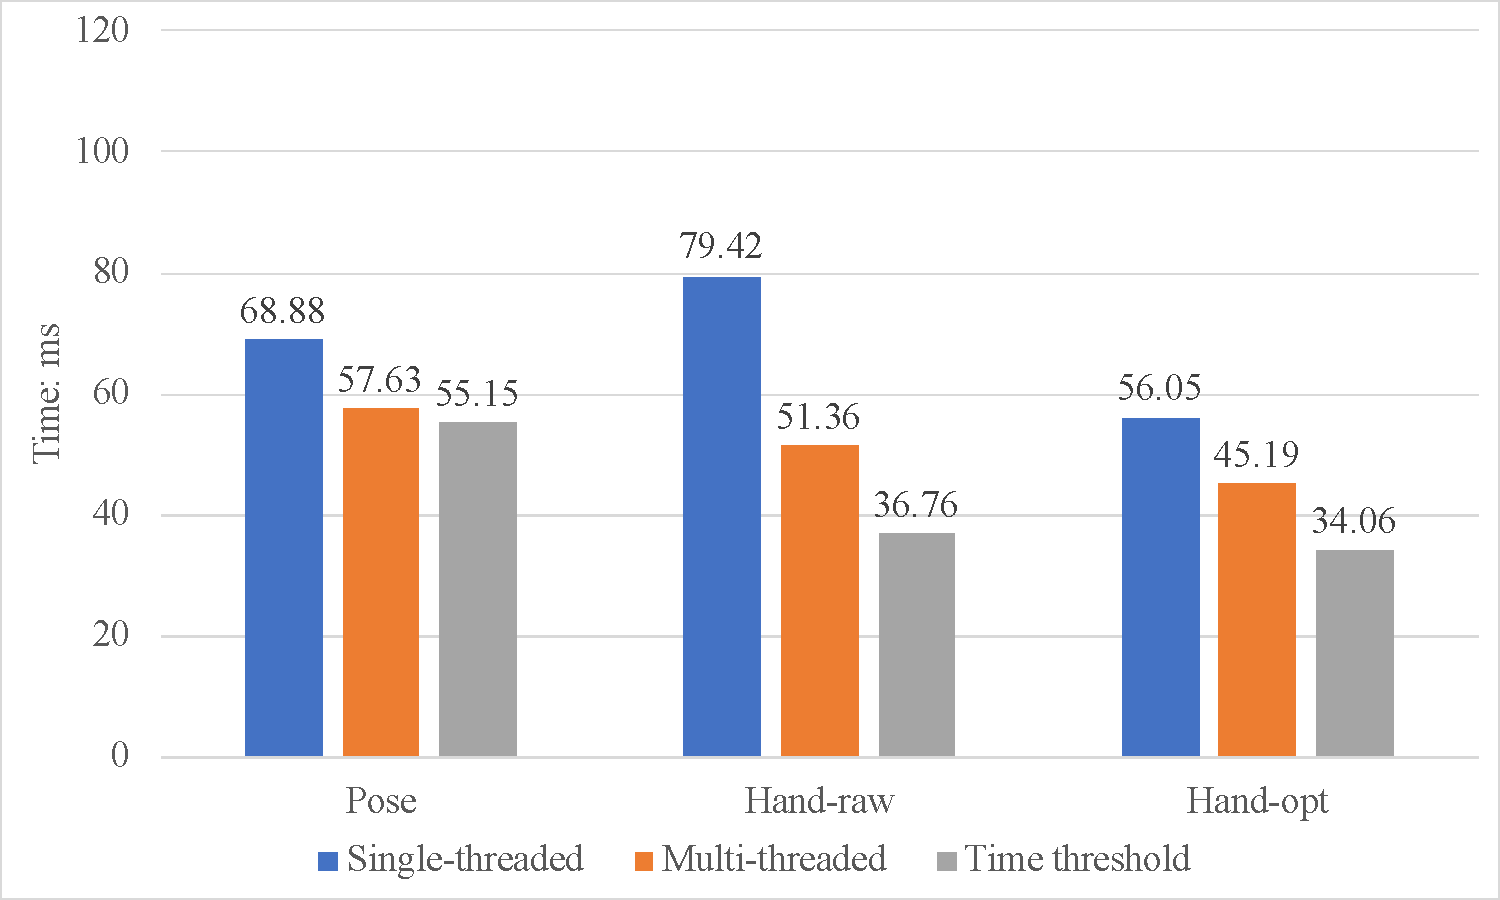
\includegraphics[width=\textwidth]{figure/win_stats.pdf}
    \caption{ThinkPad X1, i5 4-Core}
    \end{subfigure}
    \bicaption[视频处理任务在不同CPU上运行速度测试结果]{视频处理任务在不同CPU上运行速度测试结果,两个计算设备在运行测试任务过程中每帧的平均处理耗时。其中Single-threaded是未优化的单线程运行耗时,Multi-threaded是AVPipe优化后的多线程运行耗时,Time threshold是处理流程中最耗时模块的用时,代表了速度优化的上限。}{Speed testing results on different CPU.}
    \label{fig:stats}
\end{figure}

% 就线程优化程度来说
通过对比经过多线程优化与未经过优化的平均处理时长可以发现,我们的多线程优化策略能够为测试的视频处理任务的平均每帧处理耗时带来超过10ms的提升,这体现了我们所做优化的有效性。在\ref{ch4:autoMT}中我们有提到多线程优化能达到的优化上限是处理流程中最耗时模块的用时(图\ref{fig:stats}中的Time threshold列)。在测试结果中我们可以看到优化后的视频处理任务在耗时上更为接近优化上限,但与理想上限之间仍存在一定的差距。这一差距在具体任务场景下可能是由多种原因造成的,如线程管理上的开销,多线程对计算资源的竞争,流水线各阶段处理速度不同造成的线程阻塞等。
一般来说,越是复杂的处理流程越能通过优化带来更多提升,但越难接近理想优化上限;越是简单的处理流程越能接近理想优化上限,但越难获得较大的优化提升。以图\ref{fig:stats}中的任务为例,Pose任务有更简单的计算流程与模块连接,因此多线程优化空间本身就比较小,较难带来大幅度提升,但是它可以更加接近优化上限,因此Pose任务在ThinkPad上经过优化后基本可以达到与优化上限相同的耗时。
Hand-raw任务在MacBook上经过优化后在速度上有将近40ms的显著提升,但是这一优化结果与理论优化上限相比仍有近20ms的差距。Hand-raw这样的测试结果与其实际数据处理流程有着密切的关系,类似图\ref{fig:hand_dag},Hand-raw在处理每一帧时都会经过两个CNN模型的处理,而这两个CNN模型的耗时有比较接近,因此将这两个高耗时模块放在不同的线程中进行流水线并行优化即可带来较大的性能提升。而Hand-opt由于对处理流程做了算法层面的优化,减少了第一个PalmCNN模型的调用次数,降低了其在单线程上处理的耗时,也缩小了我们进行多线程优化的优化空间。\par

% 就硬件资源来说
从两个平台不同计算资源的对比上来看,拥有更好处理器配置的ThinkPad在各个测试任务中的表现均优于MacBook。从性能优化提升的相对程度上来看,ThinkPad也有着更更好的表现,如图\ref{fig:stats}中两者在Pose任务上的性能优化对比。虽然在Pose任务的优化上两台机器的线程划分均为图\ref{fig:pose_dag}中的形式存在3个线程,但两台机器在并行运行这三个线程时的额外系统控制开销并不相同。受限于处理器核心数的限制,MacBook只能使用两个核心来分配这三个线程,这必然引入了更多的计算资源竞争,从而无法达到接近优化上限的处理速度。

\section{多线程优化验证}
为了进一步确认AVPipe框架下每个线程的运行情况,同时对优化结果和理论上限之间的差距做合理解释,我们对AVPipe框架下的视频处理任务进行了运行追踪。我们在AVPipe的自动化工具中实现了利用AVPipe框架的运行记录信息(使用了glog\footnote{\url{https://github.com/google/glog}}库)来解析生成各线程的运行时间线(timeline)的脚本代码。运行log数据会被转换为格式化的json文件,供Google Chrome的Trace-viewer\footnote{\url{http://dev.chromium.org/developers/how-tos/trace-event-profiling-tool}}插件生成可视化的timeline。\par
\begin{figure}[htp]
    \centering
    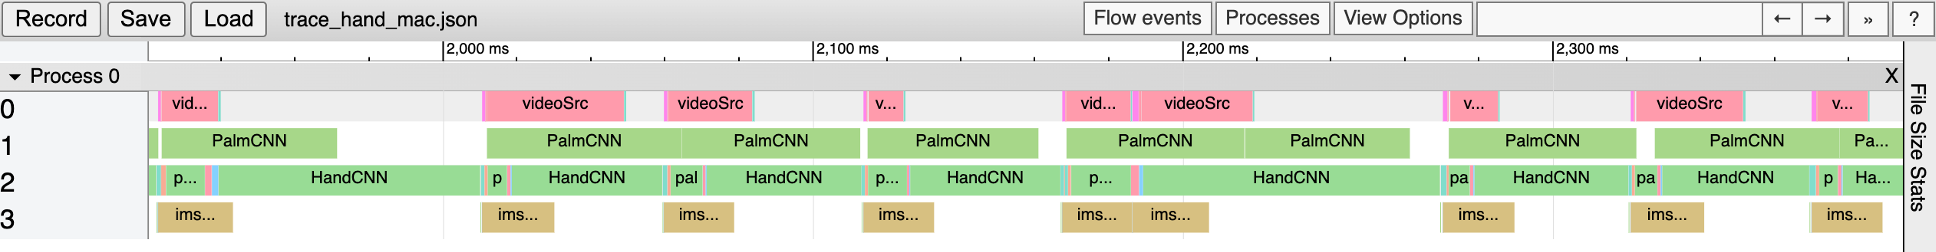
\includegraphics[width=\textwidth]{figure/trace.png}
    \bicaption[AVPipe视频处理任务的多线程时间线]{AVPipe视频处理任务的多线程时间线在Chrome Trace-viewer中的截图。图中不同横行代表不同线程,不同颜色代表不同的处理模块。该流水线是Hand-raw在MacBook上运行得到的。}{The snapshot of AVPipe task runtime timeline in Chrome Trace-viewer}
    \label{fig:trace}
\end{figure}
图\ref{fig:trace}展示了Hand-raw在MacBook上运行时的时间线。从图中可以看到PalmCNN和HandCNN这两个高耗时处理模块被分配到了两个不同的线程中运行。这两个线程也都保持着相对较高的运行负载。从图中所示的这一段运行时间来看,PalmCNN模块存在的断断续续的阻塞是由HandCNN模块无法及时处理掉PalmCNN的结果,导致PalmCNN所连接的Stream容量已满而造成的。由于HandCNN模块的输出是由PalmCNN模块的所有检测结果通过剪裁后获得的,故HandCNN的运行时的batch size是可以变化的\footnote{可以根据实际应用场景将检测数量进行固定,如每次固定只处理batch size为2的输入。},当在一些场景中人手检测数量突然增多时,HandCNN计算耗时会增长,PalmCNN的运行会因数据包堆积而阻塞。这一连串的影响最终导致了我们的优化结果无法达到理论上的优化上限。
尽管如此,高耗时模块的并行计算也确实为整个流程的处理速度带来了明显的提升。

\section{异构计算硬件下的测试}
依靠对不同神经网络推理引擎的整合,AVPipe可以支持使用如GPU,VPU等专用硬件进行深度学习的视频处理流程的构建。在本小节中,我们使用Intel GPU与Movidius VPU(NCS2)来代替以上实验中的CPU的来展示AVPipe框架的通用性与可拓展性。
值得注意的是,Intel GPU与NCS2在性能上远不及Nvidia GPU,这两者更关注功耗与便携性,故在实际性能上并没显著优于CPU。但却可以有效降低CPU的资源占用。图\ref{fig:stats_pu}展示了使用VPU和GPU的在各任务上的平均处理时长。可以看到我们的多线程优化同样为各任务的处理效率带来了提升。\par

\begin{figure}[htp]
    \centering
    \begin{subfigure}{0.49\textwidth}
    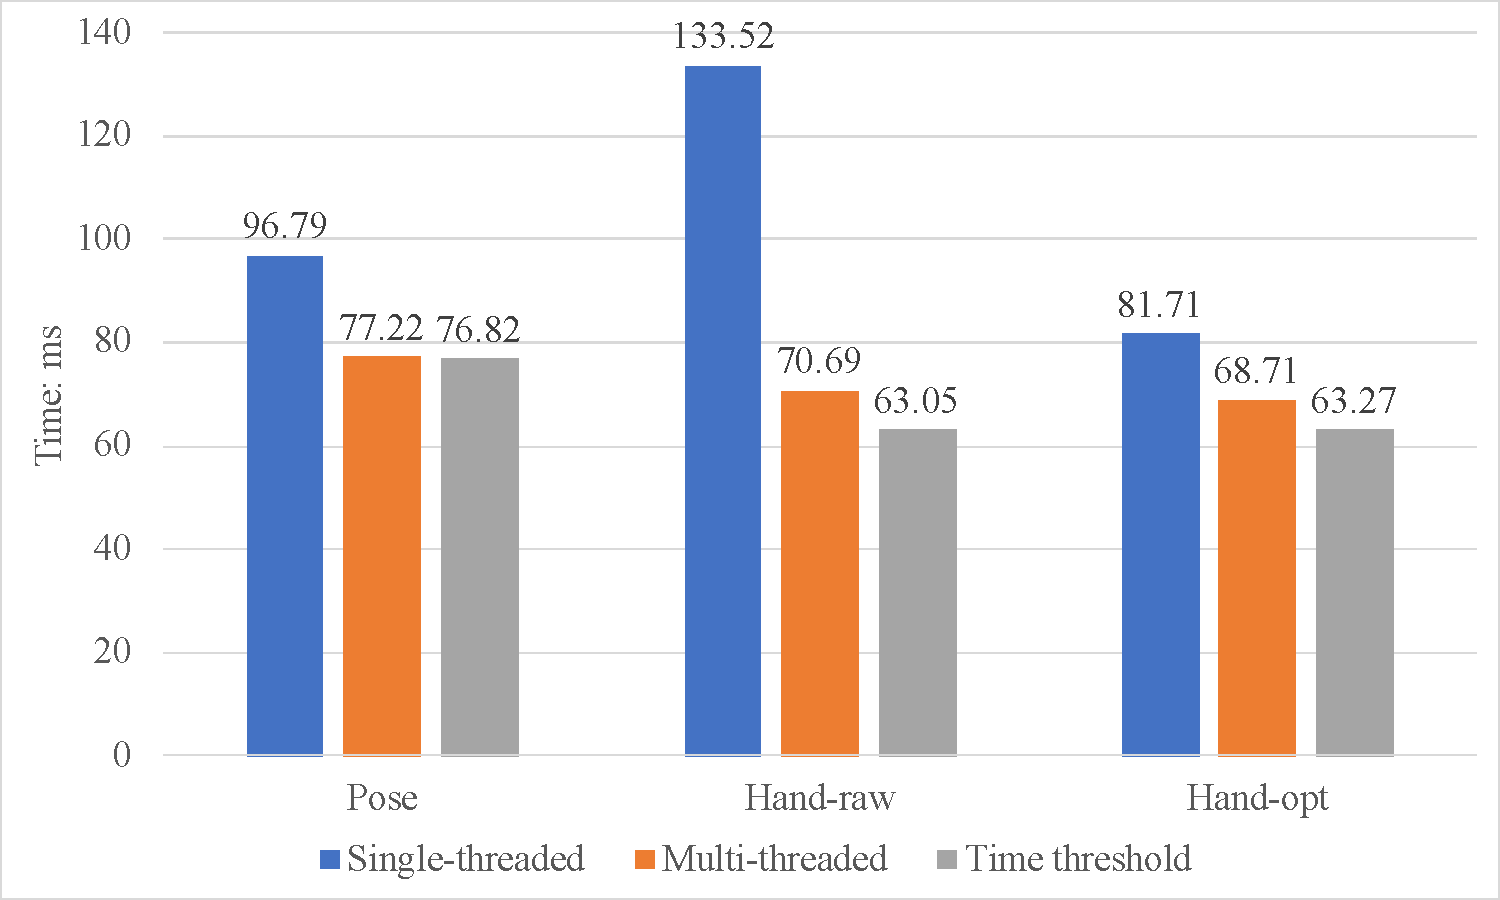
\includegraphics[width=\textwidth]{figure/VPU_stats.pdf}
    \caption{VPU, NCS2}\label{subfig:vpu}
    \end{subfigure}
    \begin{subfigure}{0.49\textwidth}
    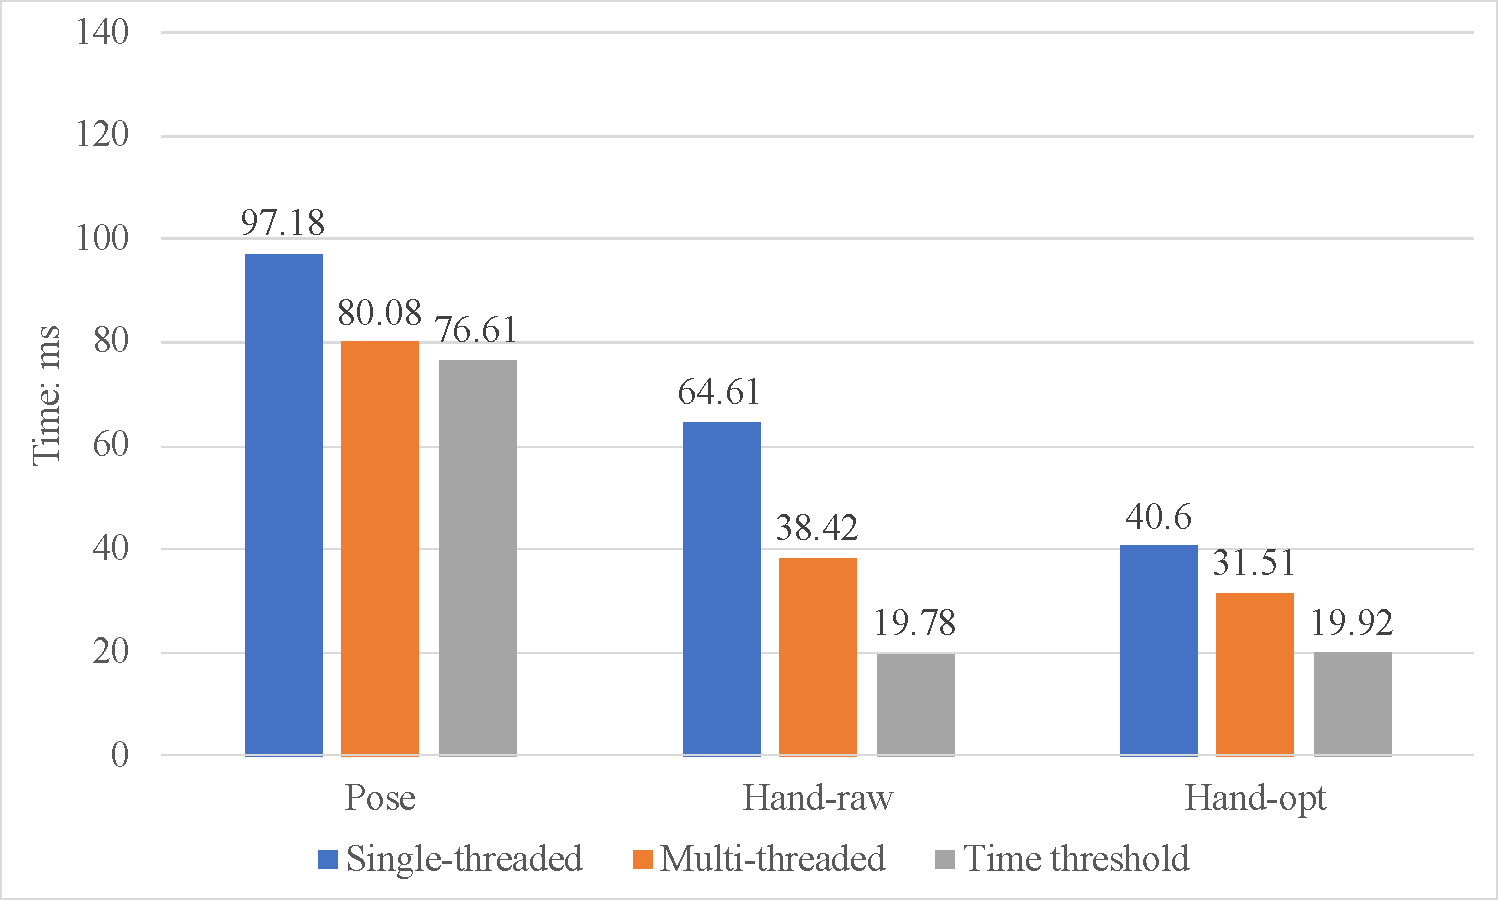
\includegraphics[width=\textwidth]{figure/GPU_stats.pdf}
    \caption{GPU, Intel Iris 540}
    \end{subfigure}
    \bicaption[视频处理任务在不同异构硬件上运行速度测试结果]{视频处理任务在不同异构硬件上运行速度测试结果。由于资源限制,VPU结果中仅PalmCNN模型部署在VPU上,HandCNN在CPU运行;而GPU测试中模型均部署在GPU上。}{Speed testing results on different heterogeneous hardware.}
    \label{fig:stats_pu}\label{subfig:gpu}
\end{figure}

Intel NCS2 VPU主要用途是为低算力的边缘设备(如Raspberry Pi)带来AI算力的提升。由于有这样的设计目标,NCS2本身就属于一个低功耗的微型处理器。因此它在CNN推理上的表现并没有强过桌面级CPU。在图\ref{subfig:vpu}展示的三个测试任务中,VPU上进行的CNN推理均为对应处理流程中最耗时的性能瓶颈模块。由于将大量计算任务分配给了VPU,这使得各线程在对CPU资源的竞争上有所缓解,我们的多线程优化也因此更能够接近VPU推理下的理论优化上限(如图\ref{subfig:vpu}中的Pose和Hand-raw任务)。虽然VPU整体表现上并没有十分突出,但结合我们提供的优化,VPU确实能为一些低算力设备带来实时AI视频流处理的能力。\par
测试视频处理任务在Intel GPU上的表现需要分情况来说明。当推理模型较大较复杂时,如Pose中用到的多路HRNet CNN模型,GPU并不能提供太多的推理加速,其实际速度甚至还会略逊于纯CPU的推理速度。但当模型是常规且简单的CNN结构时,如Hand任务中的PalmCNN和HandCNN,GPU是能够在模型推理上带来较大幅度性能提升的。这也使得经过处理算法和系统多线程优化后的Hand-opt可以达到30FPS以上的实时处理速度。在另一方面,由于Hand任务中两个CNN模型均部署在了GPU上,当多线程调用GPU进行模型推理时,必然会存在一定程度的计算资源竞争,因此我们的多线程优化很难达到单一模型速度所代表理论优化上限。

\section{本章小结}
在本章中,我们展示了几个实际视频流处理任务在AVPipe框架下的实现。然后以这些任务为例进行AVPipe的多线程优化的测试。处理在各个情况下均有提升的测试结果说明了我们提供的多线程优化策略的有效性与通用性。接下来我们又对AVPipe框架下的多线程处理任务的实际运行情况进行追踪,对AVPipe多线程优化所能带来的性能提升程度做了合理的分析与解释。最后,我们展示了AVPipe测试任务在其他异构硬件上的运行效果,由此来说明AVPipe框架的高拓展性。通过不断地进行算法层面与系统层面的优化,我们相信AVPipe在以后还能为AI视频处理任务带来更多的加速。